%\chapter{det-comp}


%%%%%%%%%%%%%%%%%%%%%%%%%%%%%%%%%%%%%%%%%%%%%%
%\section{Anode Plane Assemblies}

%%%%%%%%%%%%%%%%%%%%%%%%%%%%%%%%%%%%%%%%%%%%%%
\section{Cathode Plane Assemblies}


%\subsection{Scope, requirements and design considerations}
\subsection{Scope and requirements}

The cathode plane is located in the middle of the TPC, dividing it into two equal distance drift volumes.  It is connected to the high voltage feedthrough through a receptacle, aka the HV cup, at the east end, and biased at -180\,kV.  The cathode plane is constructed from 6 cathode plane assemblies (CPAs) to form the 7\,m $\times$ 6\,m area.  It provides the bias voltage and current to all the field cage modules (top, bottom and end wall) through electrical interconnects.  It also mechanically supports 6 pairs of top/bottom field cage modules.
The cathode plane is suspended by insulating bars from the CPA installation rail.

\fixme{Gina underlined `bias' in `bias voltage' above and in first bullet point; not sure why (Anne)}

%%%%%%%%%%%%%%%%%%%%%%%%%
%\subsubsection{Requirements}
The CPA is required to:
\begin{itemize}
\item provide equipotential surfaces at $-$180kV nominal bias voltage,
\item maintain a flatness better than 1~cm when submerged in the liquid argon,
\item be constructed of materials with comparable CTEs to that of stainless steel, 
\fixme{CTE coeff of therm expansion -- add to acronym list}
\item limit the electric field exposed to LAr to under 30~kV/cm 
\item prevent damage to the TPC, including its readout electronics, in case of a HV discharge anywhere on the cathode,
\item provide constant bias voltage and current to all attached field cage (FC) resistor divider chains,
\item support the full weight of the 4 connected top/bottom field cage modules plus a person on the bottom CPA during installation,
\item accommodate cryostat roof movement between warm and LAr-filled states,
\item be constructed in a modular form that can be easily installed in the cryostat,
\item accommodate PD calibration features, and
\item avoid any trapped volume.
\end{itemize}

%%%%%%%%%%%%%%%%%%%%%%%%%
\subsection{Design considerations}

In each single phase DUNE far detector, the cathode planes are 12\,m tall by nearly 60\,m long.  When biased to the nominal voltage of -180\,kV, each cathode plane stores more than 100\,J of energy. It is of great concern on the integrity of the detector elements, including the sensitive front end electronics, if this energy is suddenly and completely released in a high voltage discharge event.  Study has shown (DUNE docdb 1320) \fixme{cite properly} that if the entire cathode plane is made of interconnected metallic electrodes, there is significant risk of damage to the front end ASICs simply due to the charge injection through the capacitive coupling between the cathode and the anode wires when the cathode voltage is forced to ground by a high voltage discharge.  

Since  a large fraction of the stored energy on the cathode plane is determined by the operating voltage and the drift distance, reducing the drift distance and therefore the cathode voltage is an option.  However, doing so while maintaining a constant detector fiducial volume would require additional detector elements and increase cost and complexity of the system.  And this will not reduce the amount of charge injection since the voltage-capacitance product remains nearly constant between the anode and cathode planes.

Subdividing the cathode into electrically isolated partitions also reduces the total energy from a single cathode partition. However the capacitive coupling between wires and cathode will not change substantially until the partition size is comparable to the drift distance. Multiple HV feedthroughs and ports per cathode also increases the system complexity. Complete HV isolation of the cathode segments is a difficult task to achieve, if we also require the cathode plane to introduce little distortion in the drift field during normal operation of the detector. 

The solution adopted in the single phase TPC design is to make the entire cathode plane out of highly resistive material such that it has a very long discharge time constant compared to an all metal construction.  In an event of high voltage breakdown at any given location on the cathode, the sudden change in voltage only occurs in a relatively localized area.  The rest of the cathode surface maintains its original bias voltage, and gradually discharges to ground through the large resistivity of the cathode material.  This greatly reduces the instantaneous charge injection to the front end electronics.

In the single phase DUNE FD, two cathode planes are positioned roughly at 1/4 and 3/4 of the width of the TPC.  Since the cathode planes are not at the geometrical center of the cryostat, the thermal convection flow of the liquid argon will exert an unbalanced force on each cathode plane. Computerized Fluid Dynamic (CFD) study (E. Voirin FD CFD) \fixme{cite properly} shows that a pressure differential on the cathode plane of the order of $\sim$1 pascal is to be expected.  The cathode plane must be designed to withstand such pressure without exceeding the 1\,cm flatness requirement.




%%%%%%%%%%%%%%%%%%%%%%%%%
\subsection{CPA design}

%%%%%%%%%%%%%%%%%%%%%%%%%
\subsubsection{Overview}

The cathode design has evolved through several iterations over the years.  The design chosen for the ProtoDUNE-SP TPC is an array of moderately sized modules constructed from strong G10 frames holding thin G10 sheets laminated with a commercial resistive Kapton film on both sides.   Compared with the size of an APA, the CPA modules are 1/2 in width (1.16\,m) and 1/3 in height (2\,m).   Each module has four G10 bars holding a 3mm thick G10 sheet with resistive coating.  The thickness of the G10 bars is 6cm.  The surfaces of the bars facing the APAs are covered by another set of resistive G10 strip with a different bias voltage such that these G10 bars do not cause any distortion in the drift field beyond the resistive surfaces.

A CPA is constructed from the 3 modules forming a single column.  Each CPA is suspended under the cathode support rail by a single insulating G10 bar.  On the top and bottom edges of a CPA, there are two hinges supporting the partial weight of the top and bottom field cage modules.   Adjacent CPAs are aligned through pin and slot connections to maintain co-planarity while allowing minor relative vertical shift due to cryostat roof movement.

The electrical connectivity of the resistive panels vertically along each CPA is maintained by several tabs through the edge frames.  Across the columns, there is no direct electrical connection between the panels.  Instead, they are interconnected by the ``high voltage bus''. 

The high voltage bus is a loop of a high voltage cable placed along the outer edges of the entire cathode plane, hidden between the field shaping strip overhang and the main cathode resistive sheet.  This cable must be capable of withstanding the full cathode bias voltage to prevent direct arcing to (and as a result, recharging) a cathode panel having a discharge to ground. The HV bus makes redundant connections to the resistive panels across CPAs.  It also provide a low resistance path for the field cage resistive divider chains around the cathode edges.

The outer edges of the cathode plane facing the cryostat wall are populated with the same metal profiles with insulating polyethylene caps used in the field cage.  This eliminated the need for a special design of the most crucial regions of the cathode plane: the edges of the CPA now look just like the continuation of the field cage.  Since these profiles are the only objects facing grounded surfaces, they are the most likely candidates to have HV discharges to ground.   To limit peak current flow, these edge profiles are resistively connected to the main cathode panels through their laminated resistive surfaces.  


\begin{cdrfigure}[Resistive surface CPA Concept]{cpa-concept}{The resistive surface CPA concept. 
 Left: A 3D model of a corner of the cathode showing major components;  Right: E field simulation of a portion of the cathode.} 
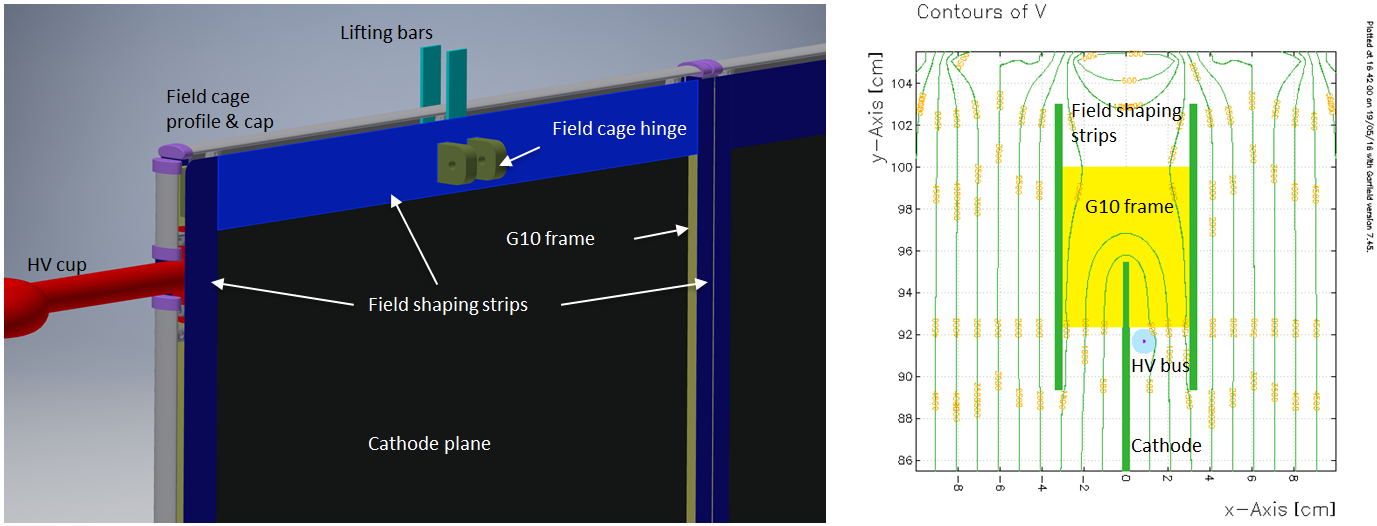
\includegraphics[width=\linewidth]{tpc_cpa_concept.png}
\end{cdrfigure}


%%%%%%%%%%%%%
\subsubsection{Resistive material}

The main criteria for the selection of the resistive material to be used for the CPA panels are: 
\begin{itemize}	
\item surface resistivity range,
\item compatibility with cryogenic temperatures,
\item robustness to HV discharges, 
\item material ageing,
\item radio-purity,
\item availability on large area, and 
\item meet the cathode flatness requirement. 
\end{itemize}



%%%%%%%%%%%%
\subsubsection{Support frame material properties}

The main material used for the cathode plane is G10. It is a thermosetting industrial fiber glass composite laminate consisting of a continuous filament glass cloth material with an epoxy resin binder. This product, first introduced in the 1950's, has characteristics of high strength, low moisture absorption, excellent electrical properties  and chemical resistance. These properties are maintained in wide temp range and under humid conditions.
NEMA G10 was the designation given to Glass Epoxy sheet composite by the National Electrical Manufacture Association (NEMA) to specify a consistent product between manufacturers. 




The bulk of G10 laminate sheet is made up of difunctional or trifunctional epoxy, and a finer glass cloth with highly temperature-resistant tetra-functional epoxy gives a high-performance outer finish. \fixme{Not sure I understand: the epoxy allows it to work at high temps; what ``performance'' is high due to the finish?}

FR4 is the brominated flame-retardant version of G10. The FR4 material can usually be used where G10 material is specified; however  
the reverse is not true. CERN requires that the material used be flame-retardant but halogen free (and therefore bromine free).  FR4 meets the flame-retardant requirement but 
is not halogen-free. Research needs to be conducted into what type of G10/FR4 is available that meets CERN's requirements.
Another variation of G10 fiberglass sheet is G10 CR laminate used in cryogenic applications. 

Both G10 and FR4 are rated at 285$^\circ$F continuous operating temperature. Because they are thermosets, no melting will occur with these grades, however charring will be observed after extended periods above this temperature rating. FR4 has a UL flammability rating of 94 V-0.


A failure criterion needs to be defined for the G10 material since it is brittle and exhibits neither ductile failure nor a defined yield stress like stainless steel.  Brittle materials typically rupture, and with a tensile strain of less than 0.05 exhibit a fractional reduction in area.  This dictates choosing a material according to 
the modified Mohr Theory of Failure, which recommends keeping the principal tensile stresses ess than the ultimate stress of the material.  See Shigley ``Standard Handbook of Machine Design,'' third edition.   Stress concentrations are also a concern for brittle materials and care should be taken to avoid sharp corners and other areas of stress concentrations.  Shigley defines stress concentration factors which are multipliers for geometric areas where stresses are higher; this is a common method for evaluating high stress areas.  


The material properties used for calculations were:

\begin{tabular}{l l}
G10: 	& \\
\hline
Thermal expansion Coefficient	&	$9.6 \times 10^{-6}$ cm/cmK	\\
Modulus of Elasticity			&	2,770ksi				\\
\vspace{0.5em}Ultimate stress				&	32ksi				\\
Stainless Steel: & \\
\hline
Thermal expansion Coefficient	&	$9.6 \times 10^{-6}$ cm/cmK	\\
Modulus of Elasticity			&	30,000ksi				\\
Yield stress					&	36ksi				\\
\end{tabular}
\fixme{check the CTE values}

%%%%%%%%%%%%
%\subsubsection{Mechanical design and stress analysis}

Figures~\ref{fig:cpa-geometry} and \ref{fig:cpa-view2} show the basic geometry of the CPA. Figure~\ref{fig:cpa-view2}a shows the block at the top of the CPA that is secured to the top cross bar and extends to the top supporting I-beam.  This strap must support the weight of four half FCs (4$\times$220 lbs) and the weight of the CPA itself (160~lbs) for a total weight of 1041~lbs. Figure~\ref{fig:cpa-hinge1} shows how the FC will be attached to the assembled CPA plane. 

\begin{cdrfigure}[CPA geometry]{cpa-geometry}{Basic geometry of the CPA array, close ups and a CPA column} 
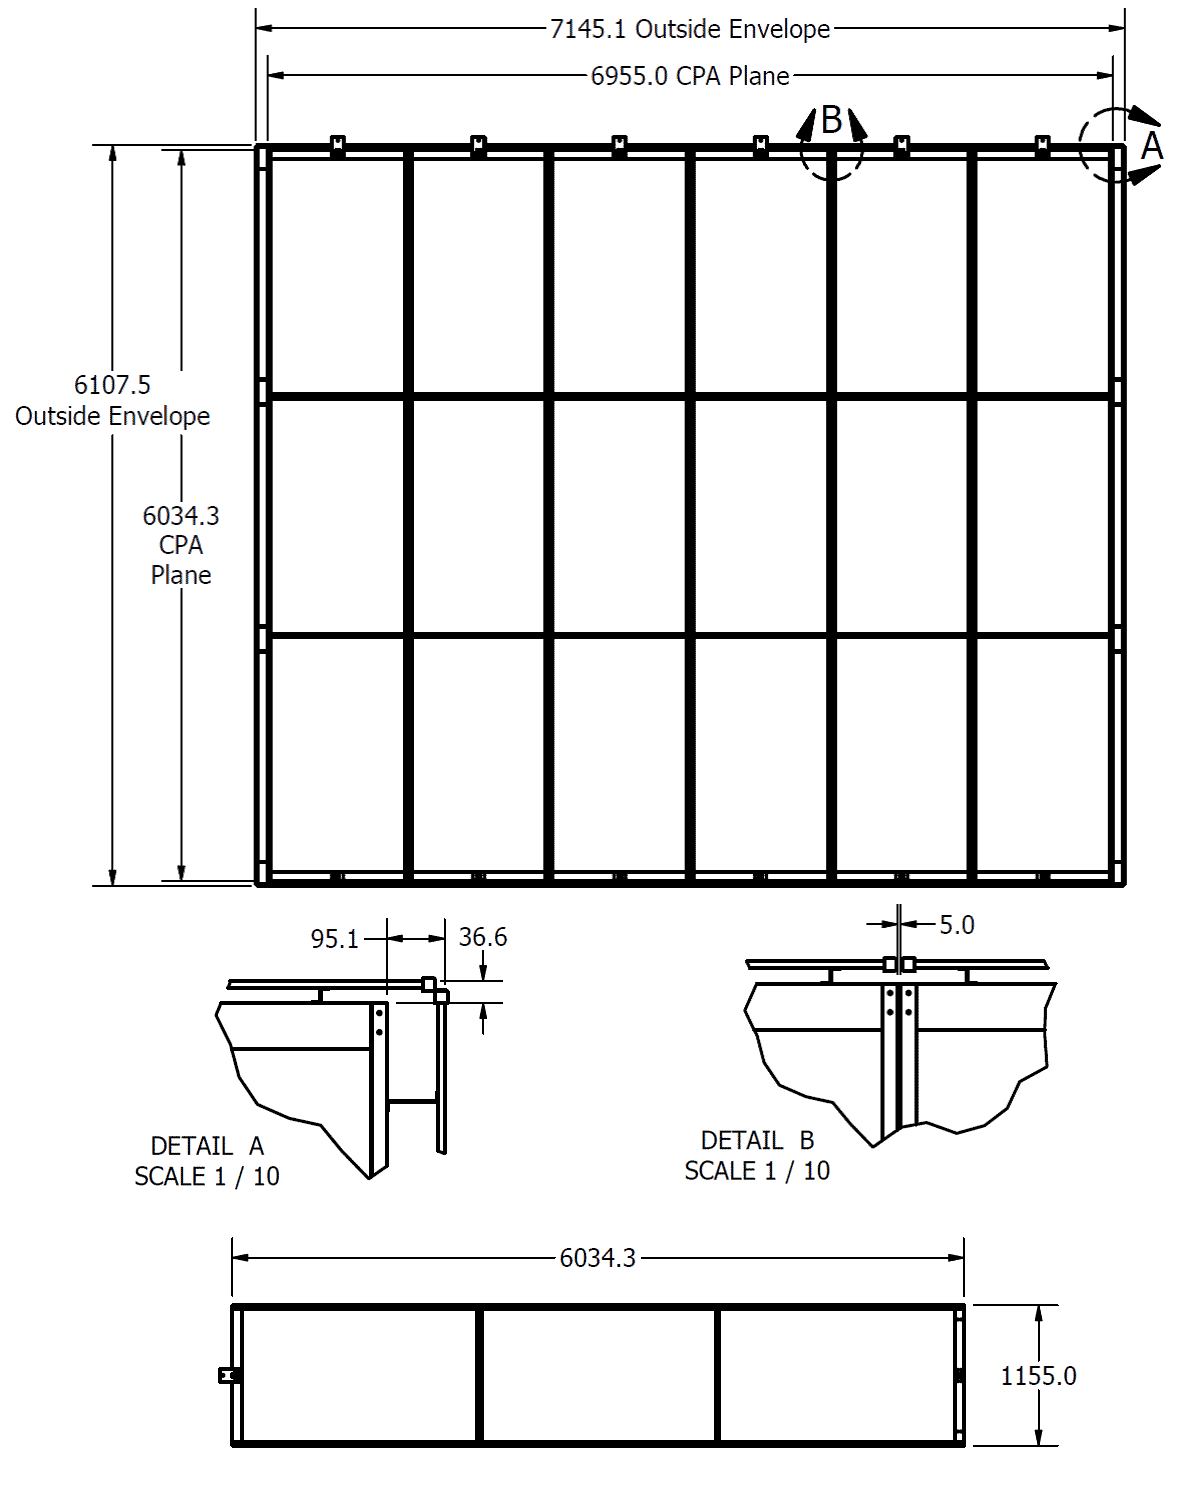
\includegraphics[width=\linewidth]{tpc_cpa_front_views1.png}
\end{cdrfigure}

\begin{cdrfigure}[CPA views2]{cpa-view2}{Views of various part of the CPAs} 
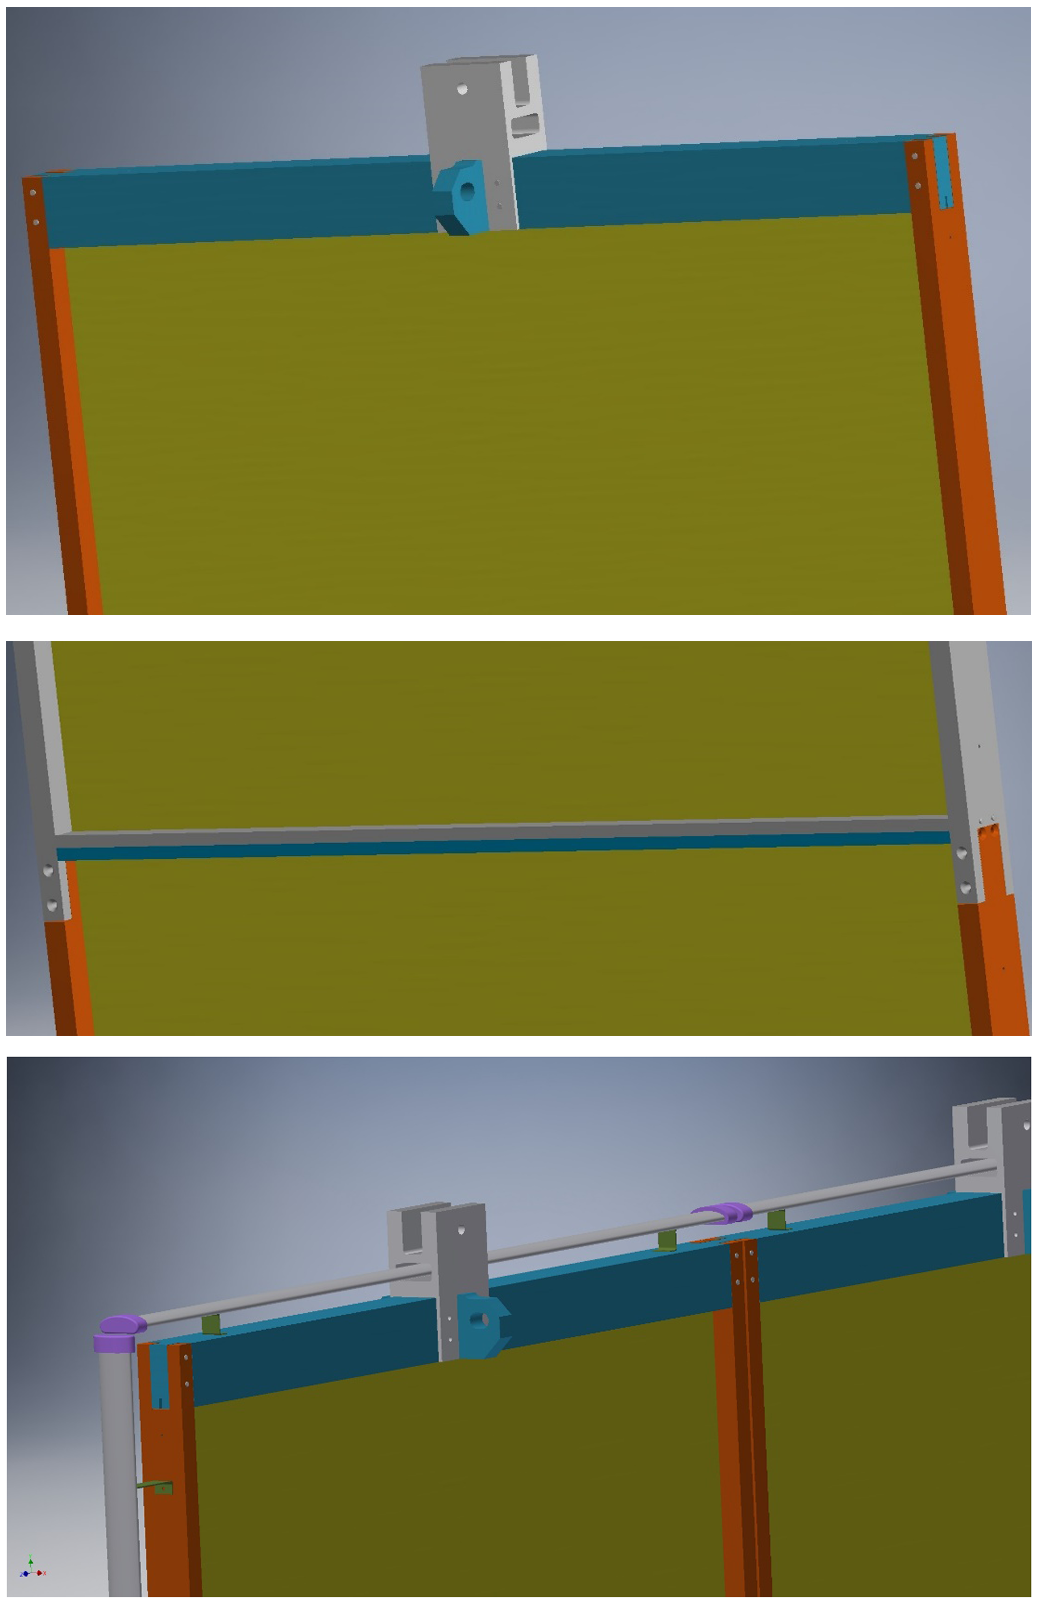
\includegraphics[width=0.8\linewidth]{tpc_cpa_views2.png}
\end{cdrfigure}

\begin{cdrfigure}[CPA and FC module hinged connection]{cpa-hinge1}{The top field cage modules are hung vertically with the CPAs when moved into the cryostat, then rotated to horizontal to attach to the APA.} 
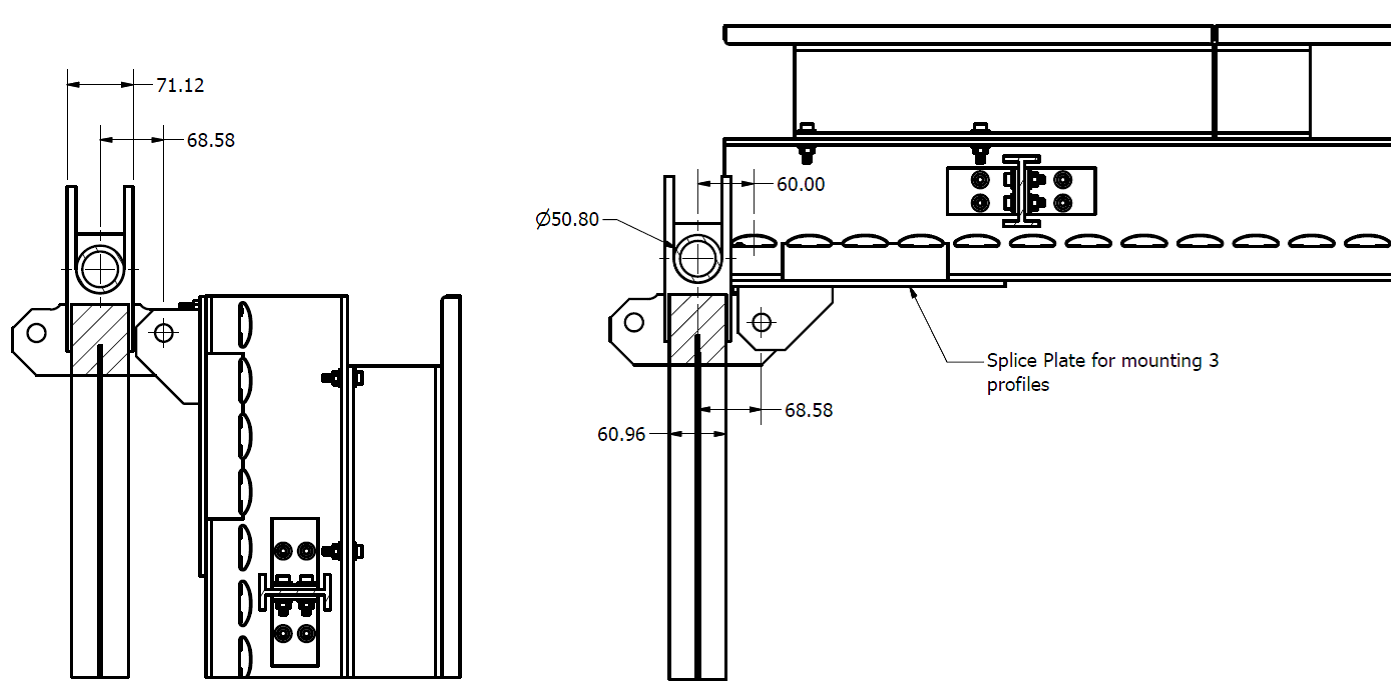
\includegraphics[width=\linewidth]{tpc_cpa_fc_hinge.png}
\end{cdrfigure}


{\it Deformation and Stress Due to Pressure from Circulating Liquid Argon}

Calculations done at Fermilab indicate that a uniform 2~Pa pressure during cool down will be applied to the resistive panels  and that this will result in 0.090~inch deflections of the panel at its center.  The CPA/FC/APA assembly will displace 8.8~mm laterally as a result of the net force from this pressure.  

{\it Thermal considerations}

When the CPA modules are cooled, their width will shrink by 0.9~mm.  The supporting stainless steel beam will shrink by 1.6~mm over the width of the CPA.  If the CPA supports are rigidly attached to the supporting stainless steel beam, then an interference of 0.7~mm (the difference) will occur.  To prevent this interference and ensure contact between CPAs after cooldown, an initial gap of 0.7~mm between CPAs is required.  

The steel beam between the CPA and APA will shrink by 5.2~mm relative to the field cage length when cooled to LAr temperature.  The joint between the FC and the CPA must be able to accommodate this shrinkage.



%%%%%%%%%%%%
\subsubsection{Mechanical and electrical interconnections between modules}

Three modules are stacked vertically to form the 6-m height of the ProtoDUNE-SP  cathode.  The frames of these modules are bolted together using tongue-and-groove connections at the ends. The resistive cathode sheets and the field-shaping strips are connected using a few metallic buttons to ensure redundant electrical contact between vertical modules.

There are six 6\,m tall CPA modules in  ProtoDUNE-SP.  Each CPA is suspended from the cathode rail using a central lifting bar.  Due to the  roof movement between the warm and cold phases of the cryostat, each column is expected to move $\sim$2~mm relative to its neighbors.  Several pin-and-slot connections are implemented at the long edges of the CPA columns to ensure the co-planarity of the modules and yet allow small vertical displacement.  The HV bus interconnects the resistive cathode surfaces across the columns to maintain a uniform voltage across the cathode surface.


